% https://www.mathworks.com/examples/matlab/mw/matlab-ex13677222-solve-nonstiff-odes

\PassOptionsToPackage{hyphens}{url}% allow line breaks at hyphens in urls
\documentclass[12pt]{matlatex}
\usepackage{examples}
\usepackage{pgfplots}
\usepackage{caption}

\begin{document}

\section*{Numerical integration of coupled ODEs}

This example is based that given in the Mathworks web page%
\ \url{https://www.mathworks.com/examples/matlab/mw/matlab-ex13677222-solve-nonstiff-odes}.
It uses the Matlab function {\tt\small ODE45} to integrate a coupled pair of ordinary differential equations -- the van der Pol equation with $\mu=1$.

\begin{matlab}
   [t,y] = ode45(@vdp1,[0 20],[2; 0]);

   % Plot of the solution
   plot(t,y(:,1),'-o',t,y(:,2),'-o')
   xlabel('Time t')
   ylabel('Solution y')
   legend('y_1','y_2')

   print(gcf,'example_02_fig.png','-dpng');

   dlmwrite ('example_02.txt',[t';y(:,1)';y(:,2)']','delimiter',' ','precision','% .8e');

   function dydt = vdp1(t,y)
   %VDP1  Evaluate the van der Pol ODEs for mu = 1
   %
   %   See also ODE113, ODE23, ODE45.

   %   Jacek Kierzenka and Lawrence F. Shampine
   %   Copyright 1984-2014 The MathWorks, Inc.

   dydt = [y(2); (1-y(1)^2)*y(2)-y(1)];
   end
\end{matlab}

\clearpage

\begin{figure}
   \centering
   \IfFileExists{example_02_fig.png}%
   {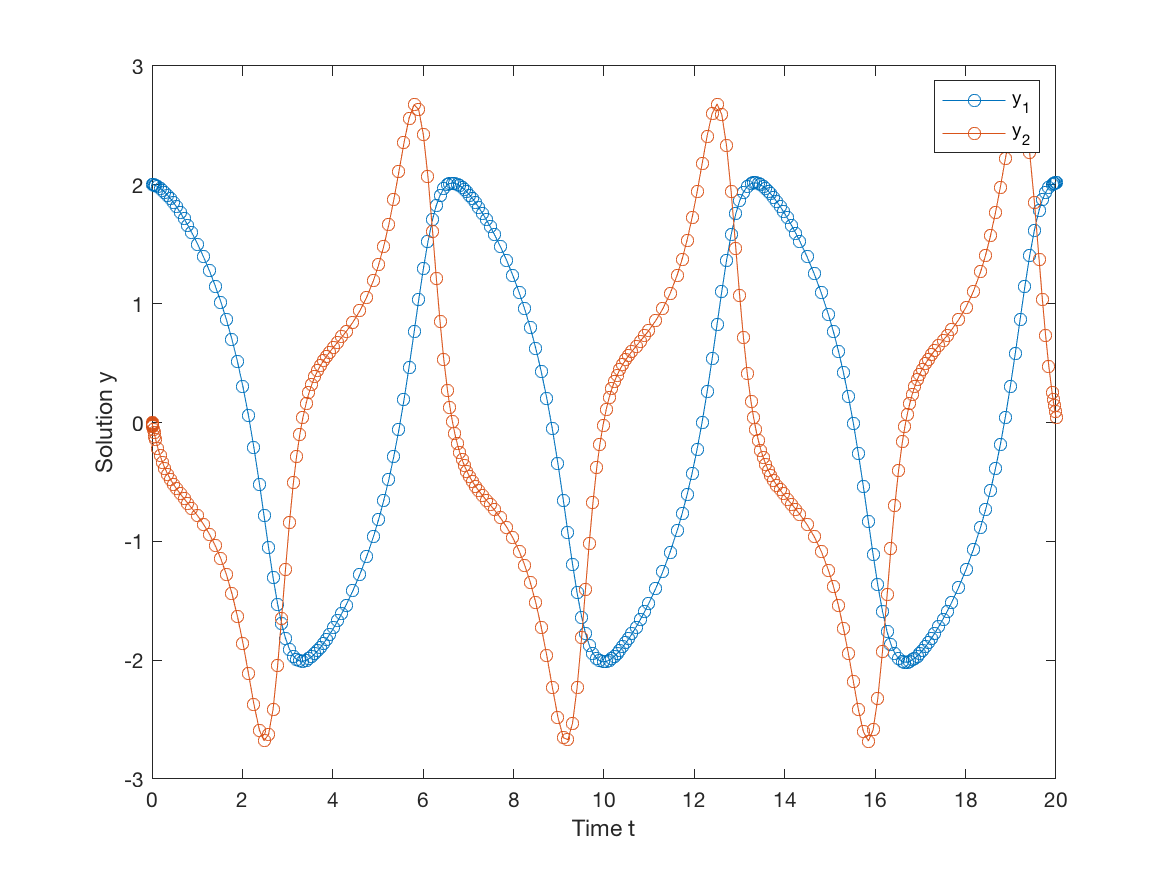
\includegraphics[width=0.75\textwidth]{example_02_fig.png}}{Failed to create png plot.}
   \caption{Solution of van der Pol equation ($\mu = 1$) using ODE45.}
\end{figure}

\clearpage

\pgfplotsset{compat=newest}
\pgfplotsset{width=0.60\textwidth,height=0.40\textwidth}

\begin{center}
   \begin{tikzpicture}
      \begin{axis}
         [xmin= 0.0, xmax=20.0,
          ymin=-3.0, ymax=3.0,
          xlabel=$\text{Time }t$, ylabel=$\text{Solution }y$,
          grid=major, grid style={dashed,gray!30},
          legend entries = {$y_1$, $y_2$}]
          \addplot[blue, mark=o]   table [x index=0, y index=1]{example_02.txt};
          \addplot[red, mark=o]    table [x index=0, y index=2]{example_02.txt};
      \end{axis}
   \end{tikzpicture}
   \captionof{figure}{Solution of van der Pol equation ($\mu = 1$) using ODE45.}
\end{center}

\vfill

\begin{latex}
   \begin{tikzpicture} % requires \usepackage{pgfplots}
      \begin{axis}
         [xmin= 0.0, xmax=20.0,
          ymin=-3.0, ymax=3.0,
          xlabel=$\text{Time }t$, ylabel=$\text{Solution }y$,
          grid=major, grid style={dashed,gray!30},
          legend entries = {$y_1$, $y_2$}]
          \addplot[blue, mark=o]   table [x index=0, y index=1]{example_02.txt};
          \addplot[red, mark=o]    table [x index=0, y index=2]{example_02.txt};
      \end{axis}
   \end{tikzpicture}
   \captionof{figure}{Solution of van der Pol equation ($\mu = 1$) using ODE45.} % requires \usepackage{caption}
\end{latex}

\end{document}
